\section{Creative Spaces}

Yale boasts a number of spaces with diverse technological audio tools and acoustic infrastructure to support the creation of new electronic and computer music.

\begin{figure}[h]
    \centering
    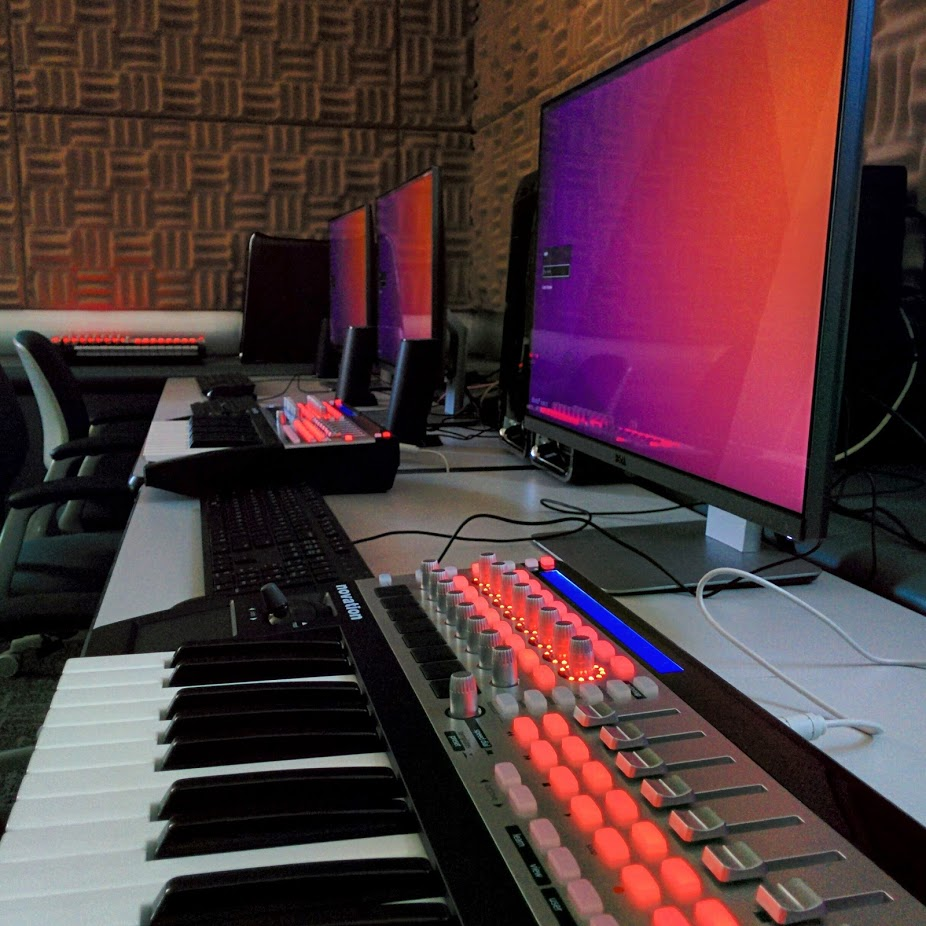
\includegraphics[width=0.85\columnwidth]{figs/euterpeastudio.png}
    \caption{The studio in AKW123}
    \label{fig:AKW123}
\end{figure}

\subsection{AKW 123}
OMI is based in the AKW 123 space in the Computer Science building. It is used to teach classes, conduct research, and host workshops and reading groups. The studio features desktop and mobile workstations for electroacoustic and new media composition built on open source synthesis and production toolchains. All workstations run a custom operating system consisting of a base Gnu-Linux OS, currently KDE Neon/Ubuntu, and a series of overlays and configurations to provide a low-latency environment with hundreds of software packages including DAWs, domain-specific audio programming languages such as SuperCollider, and a rich DSP and synthesis plugin collection. All lab machines can access the OMI server which, among other things, provides access to terabytes of sound samples.

The studio is equipped with a wide range of hardware including; digital and analog audio mixers and interfaces, 20 portable midi keyboards and miscellaneous MIDI and OSC controllers, built-in video projection, various studio microphones, field recording devices, electronic performance interfaces such as an EWI controller and a Yamaha [MODELNAMEHERE] MIDI piano, game controllers, LEAP motion sensors,VR headsets (Oculus Rift and HTC Vive), and Microsoft Kinects. The studio also owns 4 analog synthesizers: a Novation Peak, a Moog Werkstatt, a microKORG Vocoder, and a Behringer Deepmind12. These are used in OMI's ``synth jams'', as well as for student projects. The space also supplies hardware components such as Arduinos, Bela Boards, and Raspberry Pis, as well as custom built hardware interfaces like the OMIPOD~\cite{omipod}. All hardware is made available to faculty and students for their own creative practice and research. 

\subsection{Center for Collaborative Arts and Media}

Additionally, OMI benefits from the rich ecosystem for computational arts at Yale. The Center for Collaborative Arts and Media (CCAM) is the central hub for C2-related activities. The center provides physical resources such as an audio-visual post-production suite and an 8-channel, reconfigurable transdisciplinary performance space equipped with a 32 camera motion capture system. The CCAM also provides human resources in the form of workshops and lectures by visiting artists and intellectuals, as well as those from the Yale community. Collaboration is at the heart of the center which provides ample opportunities for students and faculty to work together to workshop, research and produce creative work at the intersection of the sciences, arts and technology.

\subsection{Yale Music Technology Labs}

The Department of Music houses the Yale Music Technology Labs (YalMusT) which are comprised of two teaching labs, a small post-production studio and an advanced audio technology classroom. Both labs have surround-sound systems and the studio boasts a specially calibrated Genelec monitoring system. Further details on these spaces can be found online\footnote{\url{https://yalmust.yale.edu/}}.

\subsection{Residential College Studios}

The residential college system at Yale boasts five production studios that support audio recording, editing, and production. Each facility features a different set of equipment to expose students to a variety of studio environments. Furthermore, all studios are managed by student volunteers. Further details on these spaces can be found online\footnote{\url{https://up.yalecollege.yale.edu/production-resources/music-production-facilities}}.

